\section{Architecture Integration}

\subsection{Model Support}

\begin{table}[H]
\centering
\small
\begin{tabular}{llllll}
\toprule
\textbf{Architecture} & \textbf{Attention} & \textbf{Nested?} & \textbf{RoPE?} & \textbf{GQA?} & \textbf{Cross-attn?} \\
\midrule
DistilBERT & Flat & No & No & No & No \\
RoBERTa & Nested & Yes & No & No & No \\
GPT-2 & Causal & No & No & No & No \\
Qwen3.5 & GQA+RoPE & No & Yes & Yes & No \\
T5 & Enc-Dec & No & No & No & \textbf{Yes} \\
\bottomrule
\end{tabular}
\end{table}

\subsection{Weight Extraction}

\subsubsection{DistilBERT}
\begin{lstlisting}
q\_w = src.q\_lin.weight
k\_w = src.k\_lin.weight
v\_w = src.v\_lin.weight
o\_w = src.out\_lin.weight
\end{lstlisting}

\subsubsection{RoBERTa (Nested)}
\begin{lstlisting}
q\_w = src.self.query.weight
k\_w = src.self.key.weight
v\_w = src.self.value.weight
o\_w = src.output.dense.weight  # For reference, not applied
is\_nested\_encoder = True
\end{lstlisting}

\subsubsection{GPT-2 (Fused Conv1D)}
\begin{lstlisting}
fused = src.c\_attn.weight.T
q\_w, k\_w, v\_w = fused.chunk(3, dim=0)
o\_w = src.c\_proj.weight.T
\end{lstlisting}

\subsubsection{Qwen (GQA + RoPE)}
Direct copy from \texttt{q\_proj}, \texttt{k\_proj}, \texttt{v\_proj}, \texttt{o\_proj}.

\subsection{Nested Encoder Bypass}

For RoBERTa, BAM-UMoE's \texttt{out\_lin} is not applied; the outer 
\texttt{BertSelfOutput.dense} performs the projection. This avoids double projection.

\subsection{Partial RoPE}

For Qwen3.5 with \texttt{head\_dim=256} and \texttt{rotary\_dim=64}:
\begin{lstlisting}
q\_rot, q\_pass = q[..., :rotary\_dim], q[..., rotary\_dim:]
q\_rot = (q\_rot * cos) + (rotate\_half(q\_rot) * sin)
q = torch.cat([q\_rot, q\_pass], dim=-1)
\end{lstlisting}

\subsection{Cross-Attention}

For encoder-decoder models, the MoE branch is \textbf{not applied} to 
cross-attention. The reason: cross-attention V is projected from encoder 
states, and pretrained cross-attention weights are highly calibrated. 
Injecting unaligned MoE there would disrupt alignment.

\begin{lstlisting}
if not is\_cross\_attention:
    moe\_delta\_v = self.qkv\_moe(hidden\_states).view(B, L, H, d\_h)
    v = v + 0.1 * moe\_delta\_v
\end{lstlisting}

\subsection{Registry}

\begin{lstlisting}
@ATTENTION\_REGISTRY.register("bam\_umoe")
class BAMUMoEBlock(BaseAttention):
    ...
\end{lstlisting}

\subsection{Failure Modes}

\begin{table}[H]
\centering
\small
\begin{tabular}{lll}
\toprule
\textbf{Failure} & \textbf{Detection} & \textbf{Response} \\
\midrule
Missing weights & \texttt{copy\_weights} raises & Return None \\
NaN in scores & \texttt{torch.nan\_to\_num} & Replace with 0 \\
MoE overflow & \texttt{torch.clamp} & Clamp to $\pm$65000 \\
Cross-attention MoE & Skip MoE branch & Preserve alignment \\
\bottomrule
\end{tabular}
\end{table}

\subsection{Numerical Stability}

\begin{lstlisting}

---
\end{lstlisting}

\begin{figure}[H]
\centering
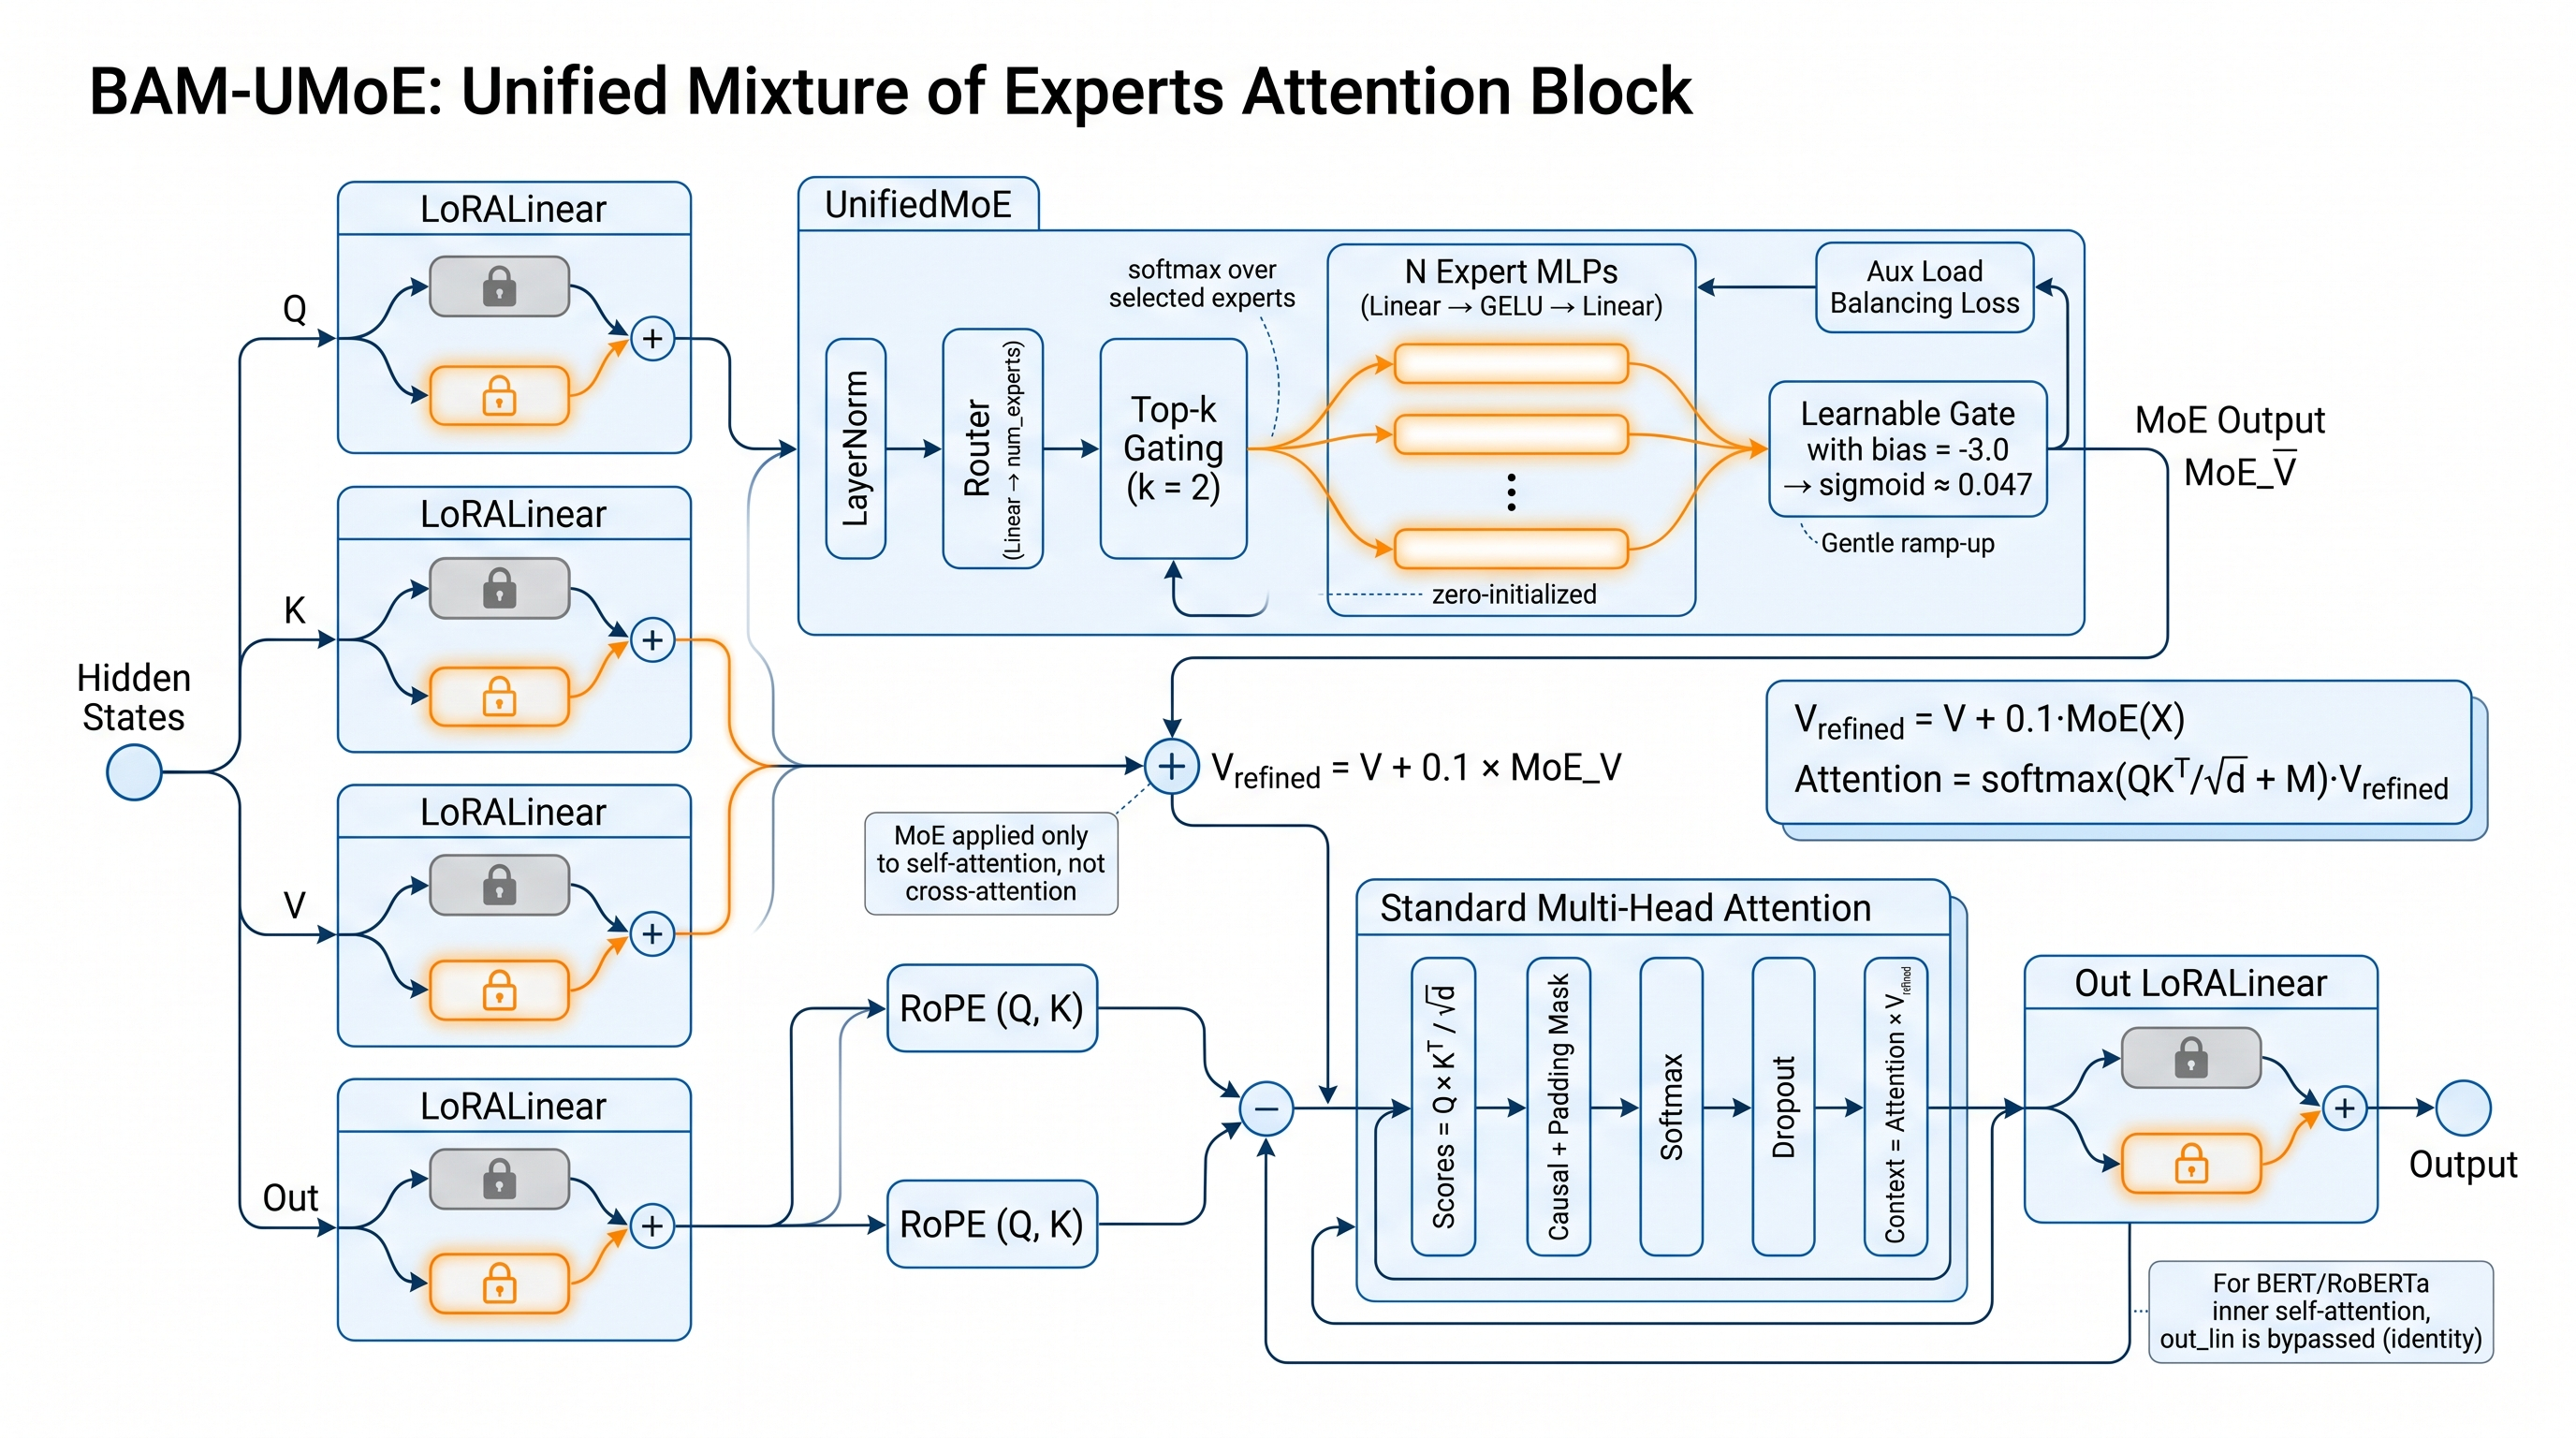
\includegraphics[width=\linewidth]{figures/architecture.jpeg}
\caption{High-level architectural diagram of bam\_umoe.}
\label{fig:arch_bam-umoe}
\end{figure}

